\draft Phonon dispersion.

\begin{parts}
	\part A phonon is a quantisation of lattice vibration due to the discrete translational symmetry in a crystal.
	Generally there are 2 branches of phonon modes, optic mode is where the neighbouring atoms are moving out of phase to one another, and acoustic mode where they oscillate in phase.
	
	\part
	\begin{subparts}
		\subpart 3D, $N$ lattice points, $p$ atoms.
		
		\subpart Space group (no longer in syllabus)
		
		\subpart Close to the BZ centre, due to the 4-fold rotational symmetry, the spectra should have degeneracy about its principal axes.
	\end{subparts}
	
	\part
	\begin{subparts}
		\subpart
		\begin{align*}
			E_i &= \SI{30}{\milli\electronvolt} \Rightarrow k_i = \frac{1}{\hbar} \sqrt{2mE_i} = \SI{3.80e10}{\per\metre} \\
			E_\textnormal{ph} &= \SI{20}{\milli\electronvolt} \Rightarrow E_f = \SI{10}{\milli\electronvolt} \Rightarrow k_f = \frac{1}{\hbar} \sqrt{2mE_f} = \SI{2.20e10}{\per\metre}
		\end{align*}
		
		So $Q = k_i - k_f$ may range from $\abs{k_i - k_f} = \SI{1.61e10}{\per\metre} = \SI{16.1}{\per\nano\metre}$ to $\abs{k_i + k_f} = \SI{6.00e10}{\per\metre} = \SI{60.0}{\per\nano\metre}$.
		
		\begin{equation*}
			|Q| = \frac{2\pi l}{c}
		\end{equation*}
		
		So for $c = 0$, we have:
		\begin{equation*}
			\abs{Q} = \begin{cases}
				\SI{14.0}{\per\nano\metre} \mtext{($l=1$, forbidden)} \\
				\SI{27.9}{\per\nano\metre} \mtext{($l=2$, allowed)} \\
				\SI{41.9}{\per\nano\metre} \mtext{($l=3$, allowed)} \\
				\SI{55.9}{\per\nano\metre} \mtext{($l=4$, allowed)} \\
				\SI{69.8}{\per\nano\metre} \mtext{($l=5$, forbidden)}
			\end{cases}
		\end{equation*}
		
		\subpart \todo
		\begin{figure}[H]
			\centering
			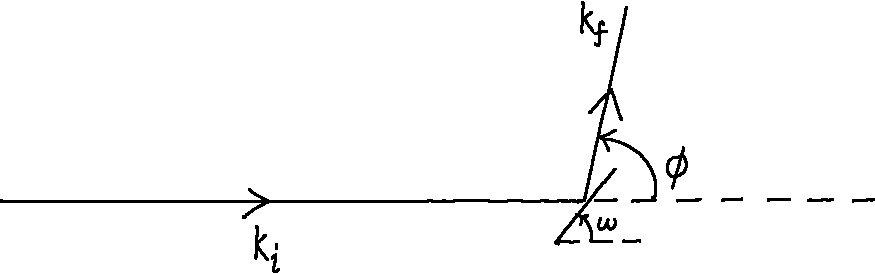
\includegraphics[width=.6\linewidth]{q1-triple-axis}
		\end{figure}
		\begin{figure}[H]
			\centering
			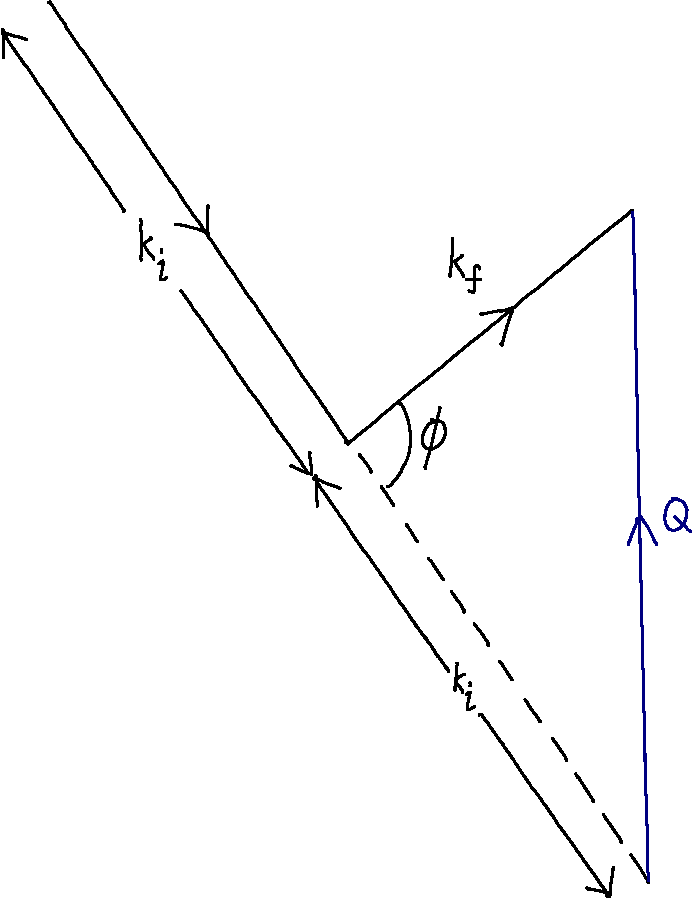
\includegraphics[width=.5\linewidth]{q1-mtm-triangle}
		\end{figure}
	\end{subparts}
\end{parts}